\documentclass{beamer}
\mode<presentation> {
%\usetheme{Madrid}
%\usetheme{default}
\usepackage{color}
\definecolor{bottomcolour}{rgb}{0.21,0.11,0.21}
\definecolor{middlecolour}{rgb}{0.21,0.11,0.21}
\setbeamercolor{structure}{fg=white}
\setbeamertemplate{frametitle}[default]%[center]
\setbeamercolor{normal text}{bg=black, fg=white}
\setbeamertemplate{background canvas}[vertical shading]
[bottom=bottomcolour, middle=middlecolour, top=black]
\setbeamertemplate{items}[circle]
\setbeamertemplate{navigation symbols}{} %no nav symbols
\setbeamercolor{block title}{use=structure,fg=white,bg=structure.fg!50!red!50!blue!100!green}
\setbeamercolor{block body}{parent=normal text,use=block title,bg=block title.bg!5!white!10!bg,fg=white}
\setbeamertemplate{navigation symbols}{}
}


\usepackage{graphicx} 
\usepackage{booktabs} 
\usepackage[utf8]{inputenc}  
\usepackage[T1]{fontenc}  
\usepackage{geometry}     
\usepackage[francais]{babel} 
\usepackage{eurosym}
\usepackage{verbatim}
\usepackage{ragged2e}
\justifying


%%%%%%%%%%%%%%%%%%%%%%%%%%%%%%%%%%%%%%%%%%%%%%%%%%%%%%%%%%%%%%%%
%% ccBeamer 0.1, 2007-07-02                                   %%
%% Written by Sebastian Pipping <webmaster@hartwork.org>      %%
%% ---------------------------------------------------------- %%
%% Licensed under Creative Commons Attribution-ShareAlike 3.0 %%
%% http://creativecommons.org/licenses/by-sa/3.0/             %%
%%%%%%%%%%%%%%%%%%%%%%%%%%%%%%%%%%%%%%%%%%%%%%%%%%%%%%%%%%%%%%%%


%% Images
\newcommand{\CcImageBy}[1]{%
	
\includegraphics[scale=#1]{creative_commons/cc_by_30.pdf}%
}
\newcommand{\CcImageCc}[1]{%
	
\includegraphics[scale=#1]{creative_commons/cc_cc_30.pdf}%
}
\newcommand{\CcImageDevNations}[1]{%
	
\includegraphics[scale=#1]{creative_commons/cc_dev_nations_30.pdf}%
}
\newcommand{\CcImageNc}[1]{%
	
\includegraphics[scale=#1]{creative_commons/cc_nc_30.pdf}%
}
\newcommand{\CcImageNd}[1]{%
	
\includegraphics[scale=#1]{creative_commons/cc_nd_30.pdf}%
}
\newcommand{\CcImagePd}[1]{%
	
\includegraphics[scale=#1]{creative_commons/cc_pd_30.pdf}%
}
\newcommand{\CcImageSa}[1]{%
	
\includegraphics[scale=#1]{creative_commons/cc_sa_30.pdf}%
}
\newcommand{\CcImageSampling}[1]{%
	
\includegraphics[scale=#1]{creative_commons/cc_sampling_30.pdf}%
}
\newcommand{\CcImageSamplingPlus}[1]{%
	
\includegraphics[scale=#1]{creative_commons/cc_sampling_plus_30.pdf}%
}


%% Groups
\newcommand{\CcGroupBy}[1]{% zoom
	\CcImageBy{#1}%
}
\newcommand{\CcGroupByNc}[2]{% zoom, gap
	\CcImageBy{#1}\hspace*{#2}\CcImageNc{#1}%
}
\newcommand{\CcGroupByNcNd}[2]{% zoom, gap
	\CcImageBy{#1}\hspace*{#2}\CcImageNc{#1}\hspace*{#2}\CcImageNd{#1}%
}
\newcommand{\CcGroupByNcSa}[2]{% zoom, gap
	\CcImageBy{#1}\hspace*{#2}\CcImageNc{#1}\hspace*{#2}\CcImageSa{#1}%
}
\newcommand{\CcGroupByNd}[2]{% zoom, gap
	\CcImageBy{#1}\hspace*{#2}\CcImageNd{#1}%
}
\newcommand{\CcGroupBySa}[2]{% zoom, gap
	\CcImageBy{#1}\hspace*{#2}\CcImageSa{#1}%
}
\newcommand{\CcGroupDevNations}[1]{% zoom
	\CcImageDevNations{#1}%
}
\newcommand{\CcGroupNcSampling}[2]{% zoom, gap
	\CcImageNc{#1}\hspace*{#2}\CcImageSampling{#1}%
}
\newcommand{\CcGroupPd}[1]{% zoom
	\CcImagePd{#1}%
}
\newcommand{\CcGroupSampling}[1]{% zoom
	\CcImageSampling{#1}%
}
\newcommand{\CcGroupSamplingPlus}[1]{% zoom
	\CcImageSamplingPlus{#1}%
}


%% Text
\newcommand{\CcLongnameBy}{Attribution}
\newcommand{\CcLongnameByNc}{Attribution-NonCommercial}
\newcommand{\CcLongnameByNcNd}{Attribution-NoDerivs}
\newcommand{\CcLongnameByNcSa}{Attribution-NonCommercial-ShareAlike}
\newcommand{\CcLongnameByNd}{Attribution-NoDerivs}
\newcommand{\CcLongnameBySa}{Attribution-ShareAlike}

\newcommand{\CcNote}[1]{% longname
	This work is licensed under the \textit{Creative Commons #1 3.0 License}.%
}


\title[Seahorse and PGP keys]{Seahorse and PGP keyss} 
\author{Genma}

\begin{document}

%% Titlepage
\begin{frame}
	\titlepage
	\vfill
	\begin{center}
		\CcGroupByNcSa{0.83}{0.95ex}\\[2.5ex]
		{\tiny\CcNote{\CcLongnameByNcSa}}
		\vspace*{-2.5ex}
	\end{center}
\end{frame}


%\begin{frame}
%\frametitle{Plan} 
%\tableofcontents
%\end{frame}

%----------------------------------------------------------------------------------------
%	PRESENTATION SLIDES
%----------------------------------------------------------------------------------------


\begin{frame}
\frametitle{
\includegraphics[scale=0.4]{./images/Genma.jpg} \ \ \  A propos de moi  }
\begin{columns}[c] 

\column{.55\textwidth} 
\textbf{Où me trouver sur Internet?}
\begin{itemize}
\item Le Blog de Genma : http://genma.free.fr
\item Twitter : http://twitter.com/genma
\end{itemize}

\textbf{Mes centres d'intérêts?}
\\ Plein de choses dont:
\begin{itemize}
\item La veille technologique
\item Le chiffrement
\end{itemize}

\column{.5\textwidth} 
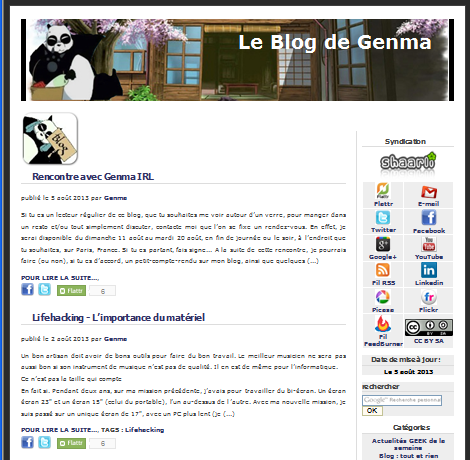
\includegraphics[width=5cm,height=5cm]{./images/blog.png} 

\end{columns}
\end{frame}


%----------------------------------------------------------------------------------------
\begin{frame}
\frametitle{Seahorse - lancement}
\begin{center}
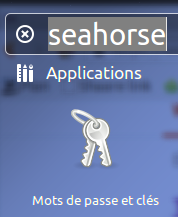
\includegraphics[scale=0.4] {./images/Seahorse00_LancementSeahorse.png}
\end{center}
\begin{itemize}\justifying{
\item Pour lancer Seahorse, il suffit de le chercher dans le dash en y tapant "Seahorse" ou "Mots de passes et clés" et de valider. 
}
\end{itemize}
\end{frame}

%----------------------------------------------------------------------------------------
\begin{frame}
\frametitle{Seahorse - premier lancement}
\begin{center}
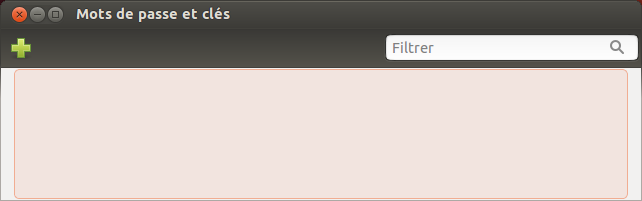
\includegraphics[scale=0.4] {./images/Seahorse01_creationclef.png}
\end{center}
\begin{itemize}
\justifying{
\item Au premier lancement, par défaut, l'interface ne contient aucune clef. On va donc en créer une.
}
\end{itemize}
\end{frame}

%----------------------------------------------------------------------------------------
\begin{frame}
\frametitle{Searhose - choix de la création d'une clef PGP}
\begin{center}
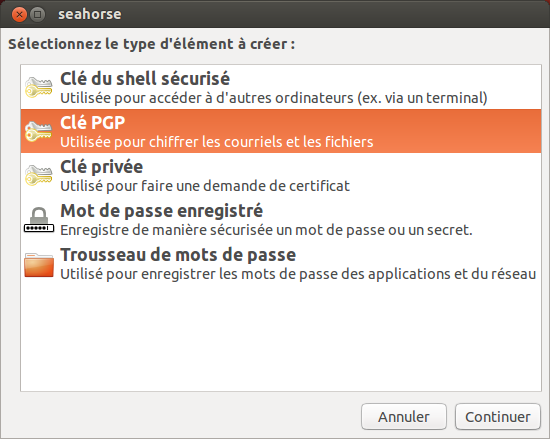
\includegraphics[scale=0.3] {./images/Seahorse02_creationclef.png}
\end{center}
\begin{itemize}
\item We will choose PGP Key	.
\end{itemize}
Rq : Seahorse permet aussi de gérer ses clefs SSH, mais ce n'est pas le but de cette présentation.
\end{frame}

%----------------------------------------------------------------------------------------
\begin{frame}
\frametitle{Searhose - informations about the user}
\begin{center}
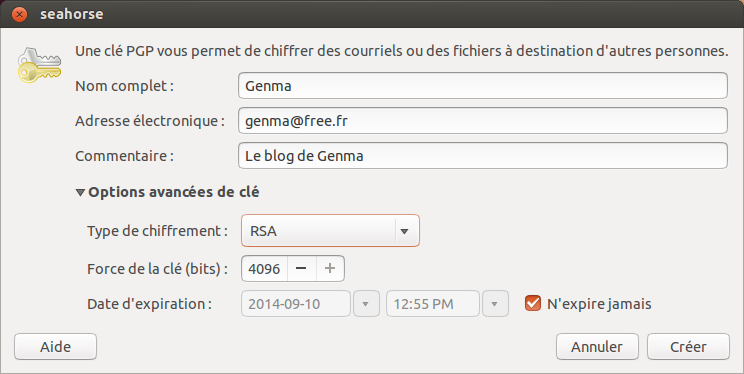
\includegraphics[scale=0.4] {./images/Seahorse03_creationclef.png}
\end{center}
\begin{itemize}
\justifying{
\item Différents champs sont à remplir.
\item Les deux options importantes sont ici la taille de la clef (4096) et la date d'expiration.
}
\end{itemize}	
\end{frame}

%----------------------------------------------------------------------------------------
\begin{frame}
\frametitle{Searhose - the passphrase}
\begin{center}
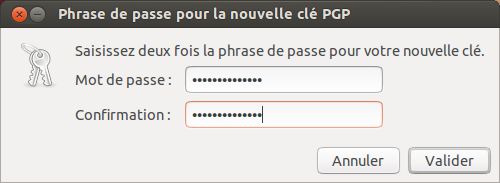
\includegraphics[scale=0.4] {./images/Seahorse04_creationclef.png}
\end{center}
\begin{itemize}
\justifying{
\item Il faut alors saisir le mot de passe qui sera utilisé par la suite à chaque utilisation de la clef. 
}
\end{itemize}
\justifying{
$\Rightarrow$  Plus le mot de passe est compliqué et long (avec des caractères spéciaux, des chiffres), mieux c'est.
\\$\Rightarrow$   ExempleDeMotDePasse*1979@
 }
\end{frame}


%----------------------------------------------------------------------------------------
\begin{frame}
\frametitle{Searhose - génération de la clef}
\begin{center}
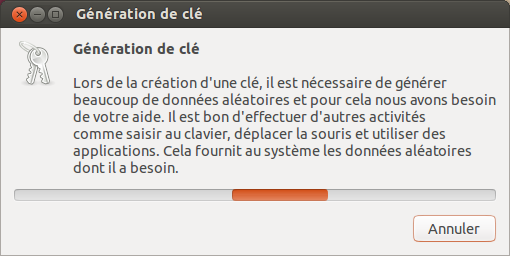
\includegraphics[scale=0.4] {./images/Seahorse05_creationclef.png}
\end{center}
\begin{itemize}
\justifying{
\item La génération de la clef commence. Comme il est conseiller de générer de l'aléatoire, personnellement, je lance la commande "ls -R /" dans un terminal.
}
\end{itemize}
\end{frame}

%----------------------------------------------------------------------------------------
\begin{frame}
\frametitle{Searhose - clef créée}
\begin{center}
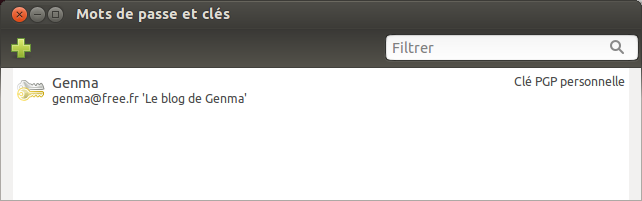
\includegraphics[scale=0.4] {./images/Seahorse06_creationclef.png}
\end{center}
\begin{itemize}
\justifying{
\item Une fois la clef créée, elle apparait dans la liste des clefs.
}
\end{itemize}
\end{frame}

%----------------------------------------------------------------------------------------
\begin{frame}
\frametitle{Searhose - détail de la clef 1/3}
\begin{center}
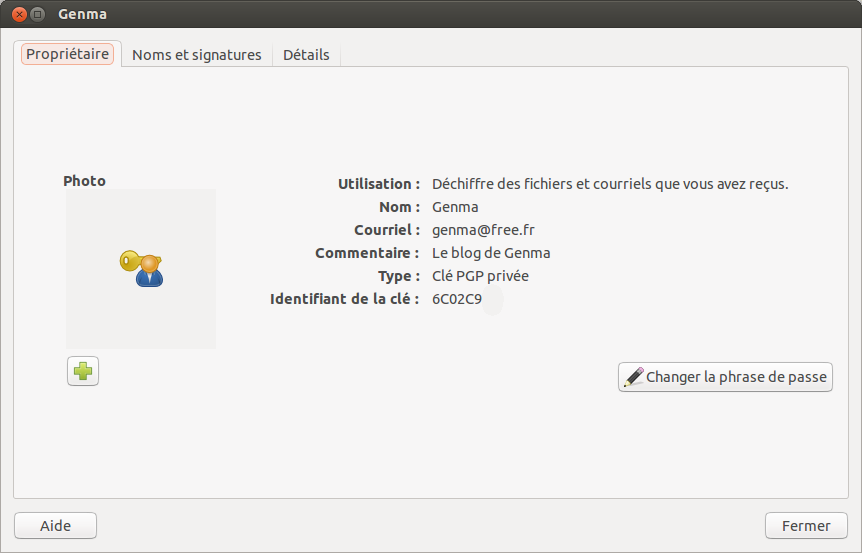
\includegraphics[scale=0.3] {./images/Seahorse07_creationclef.png}
\end{center}
\end{frame}

%----------------------------------------------------------------------------------------
\begin{frame}
\frametitle{Searhose - détail de la clef 2/3}
\begin{center}
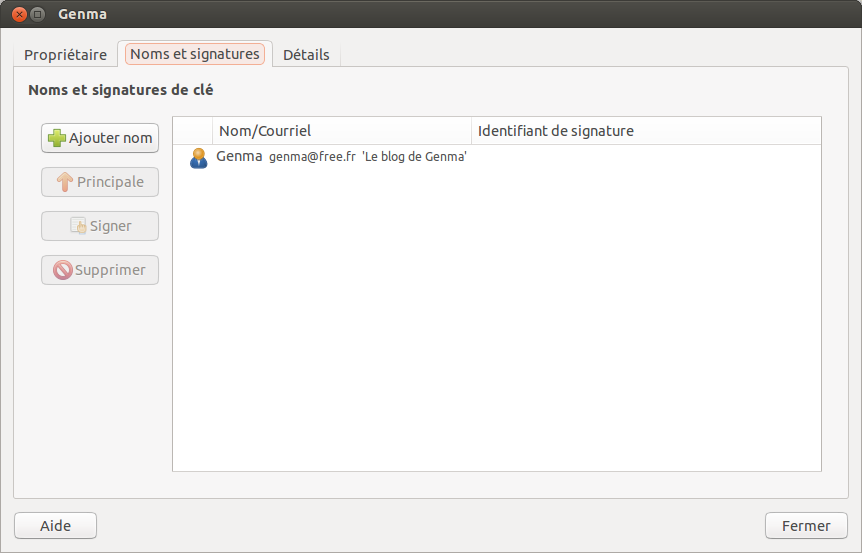
\includegraphics[scale=0.3] {./images/Seahorse08_creationclef.png}
\end{center}
\end{frame}

%----------------------------------------------------------------------------------------
\begin{frame}
\frametitle{Searhose - détail de la clef 3/3}
\begin{center}
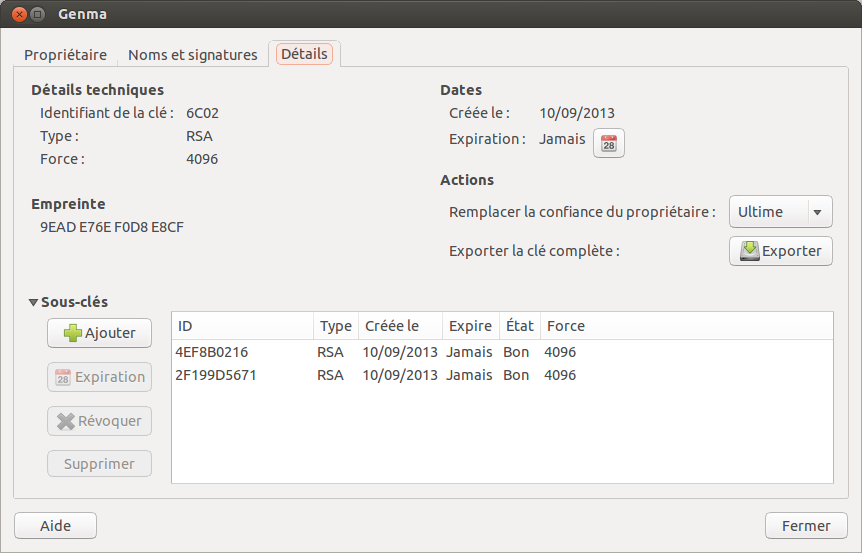
\includegraphics[scale=0.3] {./images/Seahorse09_creationclef.png}
\end{center}
\end{frame}

%----------------------------------------------------------------------------------------
\begin{frame}
\frametitle{Searhose - publication de la clef}
\begin{center}
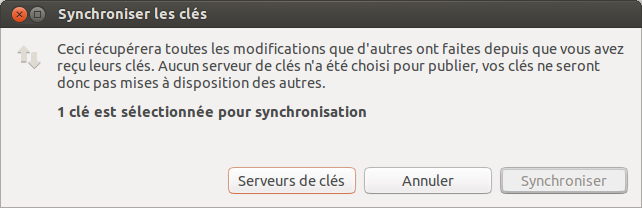
\includegraphics[scale=0.3] {./images/Seahorse_11Publicationclef.png}
\end{center}
\begin{itemize}
\justifying{
\item Pour que la clef publique soit connue et accessible à quiconque souhaite pouvoir nous envoyer un mail chiffré, il faut publier la clef sur les serveurs de clefs.
}
\end{itemize}
\end{frame}

%----------------------------------------------------------------------------------------
\begin{frame}
\frametitle{Searhose - publication de la clef}
\begin{center}
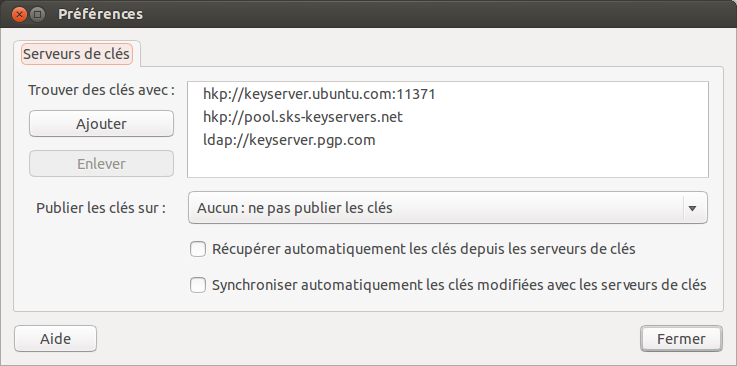
\includegraphics[scale=0.3] {./images/Seahorse_10Publicationclef.png}
\end{center}
\begin{itemize}
\justifying{
\item Il est possible de choisir les serveurs de clefs, d'en ajouter. Par défaut, les principaux sont présents.
}
\end{itemize}
\end{frame}

%----------------------------------------------------------------------------------------
\begin{frame}
\frametitle{Searhose - recherche de clefs 1/3}
\begin{center}
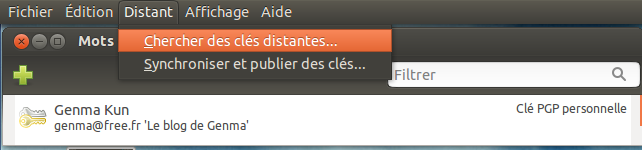
\includegraphics[scale=0.3] {./images/Seahorse_chercherclef01.png}
\end{center}
\begin{itemize}
\justifying{
\item Pour écrire à quelqu'un dont on ne connait pas encore la clef PGP, on peut rechercher sa clef publique.
}
\end{itemize}
\end{frame}

%----------------------------------------------------------------------------------------
\begin{frame}
\frametitle{Searhose - recherche de clefs 2/3}
\begin{center}
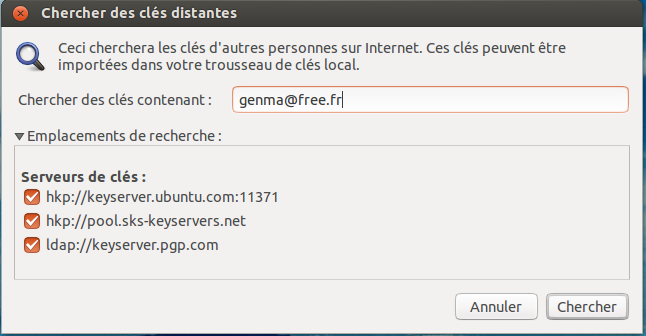
\includegraphics[scale=0.3] {./images/Seahorse_chercherclef02.png}
\end{center}
\end{frame}

%----------------------------------------------------------------------------------------
\begin{frame}
\frametitle{Searhose - recherche de clefs 3/3}
\begin{center}
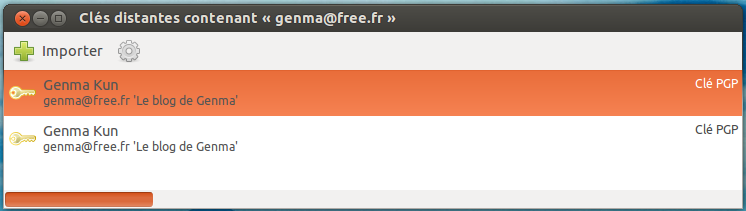
\includegraphics[scale=0.3] {./images/Seahorse_chercherclef03.png}
\end{center}
\begin{itemize}
\justifying{
\item Les clefs correspondantes sont alors proposées et on peut les ajouter à son trousseau de clefs.
}
\end{itemize}
\end{frame}

%----------------------------------------------------------------------------------------
\begin{frame}
\frametitle{Searhose - détail d'une clef publique 1/3}
\begin{center}
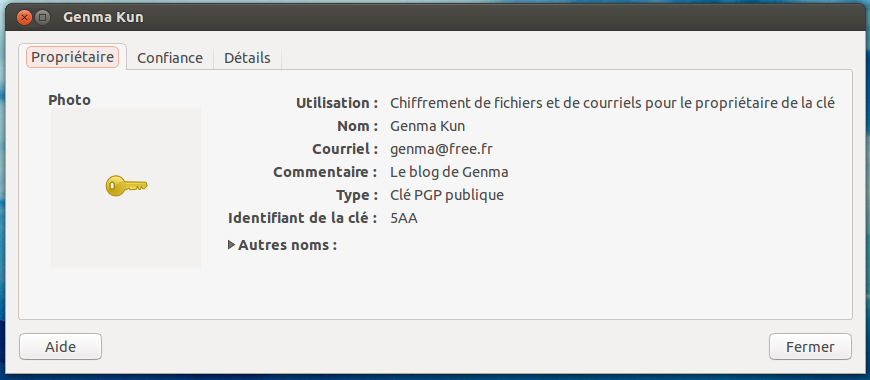
\includegraphics[scale=0.3] {./images/Seahorse_chercherclef04.png}
\end{center}
\begin{itemize}
\justifying{
\item Pour une clef publique, on peut voir les détails de la clef.
 }
\end{itemize}
\end{frame}

%----------------------------------------------------------------------------------------
\begin{frame}
\frametitle{Searhose - détail d'une clef publique 2/3}
\begin{center}
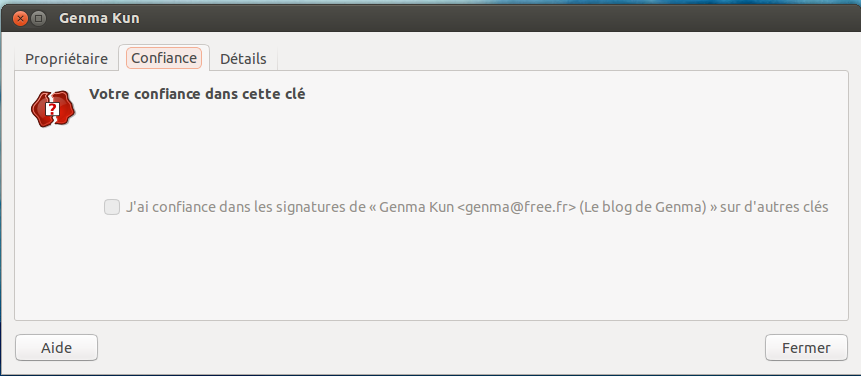
\includegraphics[scale=0.3] {./images/Seahorse_chercherclef05.png}
\end{center}
\begin{itemize}
\justifying{
\item On voit apparaitre ici la notion de confiance en la clef.
}
\end{itemize}
\justifying{
$\Rightarrow$  On valide la clef de quelqu'un lors d'une cryptopartie et on signe alors sa clef avec la notre pour dire : oui, cette clef est bien à celui à qui elle appartient.
}
\end{frame}

%----------------------------------------------------------------------------------------
\begin{frame}
\frametitle{Searhose - détail d'une clef publique 3/3}
\begin{center}
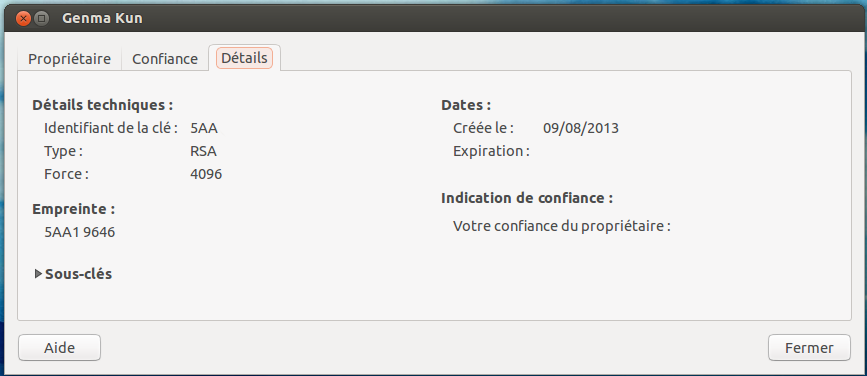
\includegraphics[scale=0.3] {./images/Seahorse_chercherclef06.png}
\end{center}
\end{frame}

%----------------------------------------------------------------------------------------
\begin{frame}
\frametitle{Searhose - gestion de son trousseau 1/2}
\begin{center}
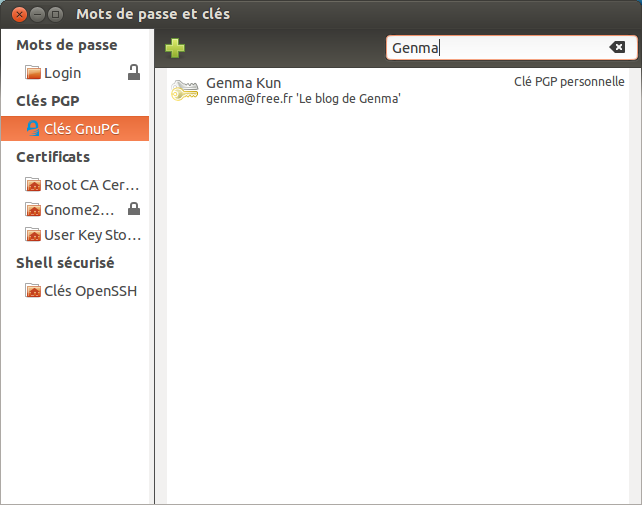
\includegraphics[scale=0.3] {./images/Seahorse_recherche_clef_contact.png}
\end{center}
\justifying{
$\Rightarrow$  Il est possible de chercher une clef dans son trousseau.
}
\end{frame}


%----------------------------------------------------------------------------------------
\begin{frame}
\frametitle{Searhose - gestion de son trousseau 2/2}
\begin{center}
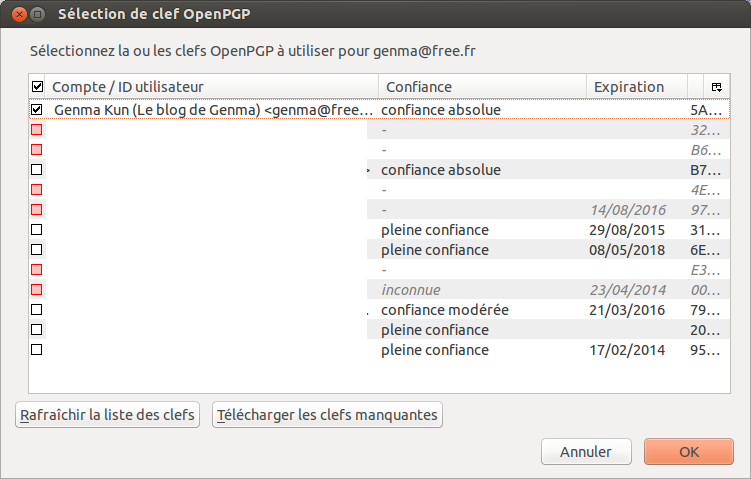
\includegraphics[scale=0.3] {./images/Searhose_liste_clefs.png}
\end{center}
$\Rightarrow$  Ou de voir toutes les clefs et la confiance que l'on a dans ces clefs.
\end{frame}

%----------------------------------------------------------------------------------------
\begin{frame}
\begin{center}
\Huge{Questions - Démonstration }
\end{center}
\end{frame}

\end{document}
